\section{结果}
\label{sec:results}

本节按证据链组织：先确认结果本身可信（\S\ref{sec:res-data}），再回答 RQ1——序列可预测性能否在独立数据集间复现（\S\ref{sec:res-replication}--\S\ref{sec:res-leakage}），然后给出边界（跨细胞系迁移、环境通道）（\S\ref{sec:res-loco}、\S\ref{sec:res-environment}），再回答 RQ2——多模型归因指认了什么、该指认能否被独立外部模型证实（\S\ref{sec:res-sequence}--\S\ref{sec:res-external}），最后回答 RQ3——该位置能否转化为可证伪的最小扰动假设（\S\ref{sec:res-counterfactual}、\S\ref{sec:res-association}、\S\ref{sec:res-evidence}）。每一小节的标题后标注其\textbf{证据层级}（E1--E6，定义见表~\ref{tab:evidence-layers}）。

\begin{figure}[htbp]
\centering
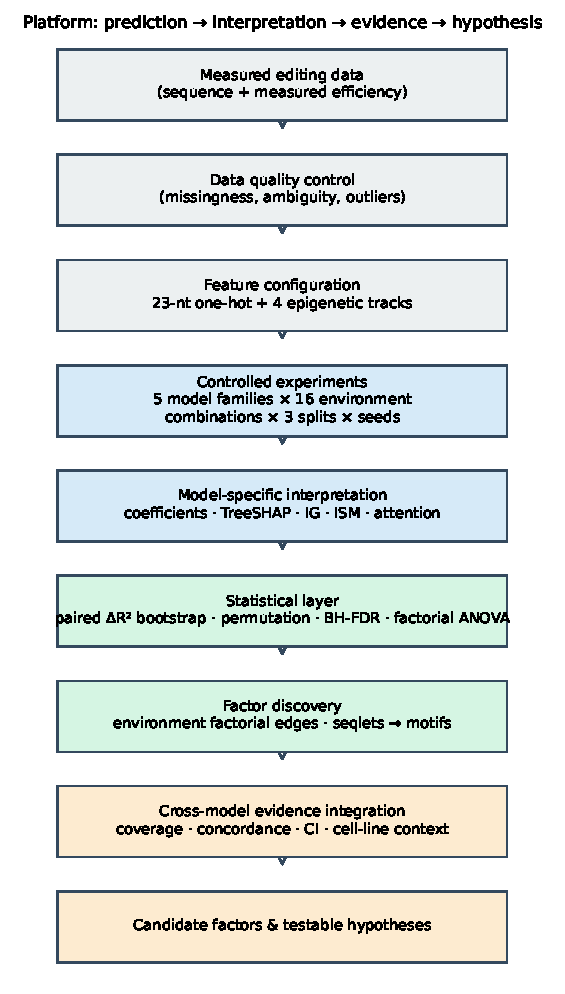
\includegraphics[width=0.5\textwidth]{figures/fig1_workflow.pdf}
\caption{平台的科学发现流程。实验测量数据依次经过质量控制、特征配置、受控多模型实验、模型特异性归因、统计与析因分析、序列模式发现、细胞背景比较、外部模型验证与跨模型证据整合，最终形成候选因素与可检验假设。各阶段之间以结构化结果文件为接口，分析阶段只读训练产物。}
\label{fig:workflow}
\end{figure}

\subsection{数据质量与泄漏防控审计（E1 前置条件）}
\label{sec:res-data}

\textbf{问题与方法.} 在报告任何模型性能之前，先确认结果本身是否可信：实验矩阵是否完整、划分是否自洽、是否存在跨划分的同源序列、全批是否运行在同一数据/代码/环境之上。

\textbf{观察（直接计算观测）.} 权威批次 \texttt{ultimate\_run} 的审计结果见表~\ref{tab:dataquality}：1\,344 次运行全部产出且可解析（\emph{single}/\emph{all}/\emph{mixed} 各 448），无 0 字节文件、无 JSON 解析失败；\textbf{1\,344 个 run 的 train$\cap$test 序列重叠与反向互补重叠全部为 0}；1\,344 次运行的划分摘要 \texttt{split\_digest} 与本地按同一代码重算的结果\textbf{逐条一致（0 处不一致）}，即训练实际使用的划分与分析阶段使用的划分完全相同；数据指纹、代码指纹、环境指纹各只有一种取值，960 个神经网络 run 全部在 GPU 上执行，无 CPU/GPU 混跑。

\textbf{口径修正的披露.} 每个 run 同时产出测试集与验证集两个指标文件。本文的全部性能数字统一取\textbf{测试集口径}。审计脚本早期版本未显式区分两者（依赖 glob 返回顺序），导致数值发散计数被记为 33；修正为显式排除验证集文件后，\textbf{测试集口径的发散 run 为 20 次（全部为 Linear Regression：\emph{single} 6、\emph{mixed} 6、\emph{all} 8）}，而 33 是验证集口径的数字。本文报告 20，并把该差异记录为口径约定的一部分（\S\ref{sec:methods-design}）。

\textbf{统计证据.} 上述为覆盖度与一致性的穷举核对（1\,344/1\,344），不涉及抽样，因此不报告 $p$ 值。

\textbf{解释（假设）与边界.} 该审计能够支持的科学陈述是：\textbf{在本文定义的身份类（序列及其反向互补）下，训练集与测试集之间不存在序列级污染，且划分在训练与分析两侧完全一致}。它\emph{不能}支持"数据中不存在任何形式的泄漏"这一更强陈述：同一 locus 的不同序列、同一细胞系内的批次效应、以及公共数据集合本身的组成偏差均不在该检查的覆盖范围内。

\textbf{数据集与实验空间.} 三个数据集的组成与划分规模见表~\ref{tab:dataset}。DeepCRISPR 过滤后保留 16\,749 条 23\,nt 序列（HCT116 4\,239、HEK293T 2\,333、HeLa 8\,101、HL60 2\,076），四个细胞系的平均归一化效率接近（0.232--0.257）。全部记录的第 22、23 位均为 G，据此确定 PAM 位于第 21--23 位。DeepCRISPR 的设计空间为 7 个模型配置 $\times$ 16 个环境组合 $\times$ 12 个（划分，种子）设定 = 1\,344 次运行；两个外部复现数据集各运行 7 个模型配置的 \emph{single} 划分。

\begin{table}[htbp]
\centering
\footnotesize
\caption{数据质量与泄漏防控审计（\texttt{ultimate\_run}）。全部数值由 \texttt{deploy/hpc/verify\_hpc\_rerun.py} 生成，逐 run 明细见 \texttt{results/tables/audit/ultimate\_run\_verify\_runs.csv}。该审计用于确认结果可信度，先于任何模型性能与科学结论报告。}
\label{tab:dataquality}
\begin{tabular}{lll}
\toprule
审计项 & 结果 & 含义 \\
\midrule
计划实验数 & 1344 & 实验矩阵完整（single/all/mixed 各 448/448/448） \\
可解析 run & 1344 & 每个 run 均含 info 与测试集 metrics；无 0 字节文件 \\
划分一致性 (split\_digest) & 12 组 / 1344 次复核 0 不一致 & 训练所用划分 == 分析所用划分 \\
序列重叠 (train$\cap$test) & 1344/1344 为 0 & $\min(\mathrm{seq},\mathrm{revcomp})$ 身份类不跨划分 \\
反向互补重叠 & 1344/1344 为 0 & L5 近重复不跨划分 \\
数据指纹 & 1 组 & 全批使用同一份数据 \\
代码指纹 & 1 组 & 全批使用同一版代码 \\
环境指纹 & 1 组 & 全批同一数值栈 \\
GPU 运行数（神经网络模型） & 960 & 无 CPU/GPU 混跑 \\
数值发散 run（$|R^{2}|\ge10$） & 20（全部为 Linear Regression） & 隔离而非删除，统计中单列 \\
\bottomrule
\end{tabular}
\end{table}

% 本文件由 analysis/reporting/paper_rewrite/build_rewrite_tables.py 自动生成。
% 请勿手工编辑；数字来源见文件头注释与 results/paper_rewrite/authoritative_numbers.json。
\begin{table}[htbp]
\centering
\footnotesize
\caption{三个数据集的组成与划分规模。DeepCRISPR 为本文的主数据集（4 个细胞系，含 4 条表观遗传通道）；Hiranniramol 与 Labuhn 为\textbf{外部复现数据集}，仅有序列通道。三者使用同一套特征构造、模型配置与评估脚本；标签均已归一化到 $[0,1]$（Hiranniramol 原始为百分制、Labuhn 为 \texttt{KO\_reporter\_assay}，由适配器统一）。划分规模按 \emph{single} 划分（70\%/15\%/15\%，身份类整体分配）报告。}
\label{tab:dataset}
\begin{tabular}{lrrrl}
\toprule
dataset / cell line & $n$ & 均值 & 标准差 & $n_{\text{train}}$ / $n_{\text{valid}}$ / $n_{\text{test}}$ \\
\midrule
\multicolumn{5}{l}{\textit{DeepCRISPR（主数据集；4 条表观通道，16\,749 条 23\,nt 序列）}} \\
HCT116 & 4\,239 & 0.254 & 0.172 & 2968 / 635 / 636 \\
HEK293T & 2\,333 & 0.238 & 0.120 & 1633 / 345 / 355 \\
HeLa & 8\,101 & 0.257 & 0.182 & 5669 / 1215 / 1217 \\
HL60 & 2\,076 & 0.232 & 0.114 & 1453 / 311 / 312 \\
\midrule
Total & 16\,749 & 0.250 & 0.165 & 11\,723 / 2\,506 / 2\,520 \\
\midrule
\multicolumn{5}{l}{\textit{外部复现数据集（仅序列通道）}} \\
Hiranniramol & 1\,309 & 0.692 & 0.371 & 916 / 196 / 197 \\
Labuhn & 417 & 0.672 & 0.248 & 291 / 63 / 63 \\
\bottomrule
\end{tabular}
\end{table}


\subsection{跨数据集复现：序列可预测性是数据集依赖的（E1）}
\label{sec:res-replication}

\textbf{问题与方法（RQ1）.} 这是本文的第一研究问题。在\textbf{完全相同的}特征构造、模型配置、身份类划分与评估脚本下，序列可预测性在三个相互独立的公开数据集上是否复现？我们同时报告两个外部数据集的结果，其中一个成功、另一个失败。为避免只比较"某一次划分下的测试 $R^{2}$"可能把"该划分恰好困难"误读为"数据无信号"，我们对每个外部数据集额外做一次\textbf{与官方划分完全无关}的复核：在全数据上用同一套 92 维特征做 5 折交叉验证，并以 200 次标签置换构造零分布（\S\ref{sec:methods-stats}）。

\textbf{观察 1（三个数据集给出三个截然不同的结论）.} 结果见表~\ref{tab:replication}。

\begin{itemize}
\item \textbf{DeepCRISPR（主数据集）}：\emph{single} 划分下 7 个配置的中位 $R^{2}$ 仅为 $0.067$--$0.120$（XGBoost 最高 0.120，CNN $k{=}3$ 最低 0.067），中位 Pearson $0.273$--$0.349$。即：信号为正但\textbf{幅度有限}。
\item \textbf{Hiranniramol（复现成功）}：在完全相同的流程下，7 个配置的测试 $R^{2}$ 为 $0.345$--$0.489$，Pearson 为 $0.607$--$0.709$。Transformer 最高（$R^{2}=0.489$，Pearson $=0.709$，Spearman $=0.665$），CNN $k{=}3$ 最低（$R^{2}=0.345$）。\textbf{所有 7 个配置均优于 DeepCRISPR 上最好的配置。}
\item \textbf{Labuhn（复现失败）}：7 个配置的测试 $R^{2}$ \textbf{全部为负}，范围 $-0.725$（Linear）至 $-0.050$（Transformer），Pearson 为 $-0.012$--$0.165$。负 $R^{2}$ 意味着模型的预测\textbf{不如直接用测试集均值}。
\end{itemize}

\textbf{观察 2（独立复核确认上述差异不是划分造成的）.} 与官方划分无关的全数据 5 折交叉验证给出同向结论：Hiranniramol 的 CV $R^{2}=+0.389$，而其标签置换零分布为 $-0.467\pm0.038$（$n=200$），两者相差 $+0.855$，即信号远超零分布；Labuhn 的 CV $R^{2}=-0.144$，其自身零分布为 $-0.287\pm0.050$，两者仅相差 $+0.143$。换言之，\textbf{Labuhn 在这个与划分无关的检验中也没有表现出可用的序列信号}。

\textbf{观察 3（Labuhn 的失败机制可诊断：预测坍缩而非标签无方差）.} 一个自然的怀疑是"Labuhn 标签方差太小，$R^{2}$ 因而不可靠"。该怀疑被数据排除：Labuhn 测试集标签标准差为 $0.215$（范围 $0.125$--$0.941$），与 Hiranniramol 的 $0.367$ 同量级。真正的原因是\textbf{预测分布的形态}（表~\ref{tab:collapse}）：

\begin{itemize}
\item Hiranniramol：7 个配置的预测标准差与标签标准差之比为 $0.67$--$0.83$，模型确实展开了预测范围并与真值相关（$r=0.61$--$0.71$）；
\item Labuhn：\textbf{6/7 个配置的该比值为 $0.03$--$0.37$}——Transformer 的预测标准差仅 $0.0070$（标签为 $0.2153$），XGBoost 为 $0.0158$，即模型把预测\textbf{压缩成了接近常数}，因此 $R^{2}$ 必然为负；
\item 唯一的例外是 Linear：其比值为 $0.93$（预测范围几乎与标签同宽），但与真值的相关仅 $r=0.165$，因此它的"方差"全是误差，反而给出了最差的 $R^{2}=-0.725$。
\end{itemize}

两种失效模式不同（坍缩 vs 方向错误），但都指向同一结论：在这 291 条训练样本上，序列特征与 Labuhn 标签之间\textbf{没有可被这批模型捕获的稳定关系}。

\textbf{观察 4（数据集间规模与标签差异不足以解释全部差异）.} 三个数据集的规模差异很大（16\,749 / 1\,309 / 417）。规模可以解释"小数据集更难"，但不能解释\textbf{方向}：Labuhn（417 条）与 Hiranniramol（1\,309 条）同属小规模、同为单细胞系、同为仅序列通道，却给出了符号相反的结论。因此本文的 RQ1 结论是：\textbf{序列可预测性的幅度乃至符号是数据集依赖的，不能被假定为跨数据集可移植的性质}。

\textbf{统计证据.} 观察 2 的置换检验（$n=200$）提供了零分布；观察 1 的每个数据集只有一次 \emph{single} 划分，因此本文不对数据集间的 $R^{2}$ 差异做显著性检验，仅报告点估计、零分布位置与失效机制的分解。

\textbf{解释（假设）与边界.} 本文\textbf{不}主张"Labuhn 上不存在任何序列效应"。可能的解释包括：该 library 的效率变异主要由序列之外的因素（染色质状态、转染效率、测定噪声）主导；291 条训练样本不足以支撑 69 维特征的拟合；或该数据集的 sgRNA 序列空间分布与 Hiranniramol / DeepCRISPR 不同。上述均为\textbf{待检验假设}。可以确定的只是本文的检验结果：\emph{在该数据集与该流程下未检出可用的序列可预测性}。

\begin{table}[htbp]
\centering
\scriptsize
\caption{Labuhn 与 Hiranniramol 的预测分布形态（测试集口径）。$\mathrm{sd}_{\text{pred}}/\mathrm{sd}_{y}$ 为预测标准差与标签标准差之比：接近 1 且相关系数为正表示模型展开了合理范围，接近 0 表示预测坍缩。Labuhn 的 6/7 个配置发生坍缩；Linear 未坍缩但与真值不相关（$r=0.165$），故 $R^{2}$ 最低。}
\label{tab:collapse}
\begin{tabular}{llrrr}
\toprule
dataset & model & $\mathrm{sd}_{y}$ & $\mathrm{sd}_{\text{pred}}$ & $\mathrm{sd}_{\text{pred}}/\mathrm{sd}_{y}$ \\
\midrule
\multicolumn{5}{l}{\textit{Hiranniramol}（$n_{\text{test}}=197$）} \\
 & Transformer & 0.3674 & 0.3034 & 0.83 \\
 & CNN $k{=}3$ & 0.3674 & 0.2774 & 0.76 \\
 & MLP & 0.3674 & 0.2648 & 0.72 \\
 & CNN $k{=}7$ & 0.3674 & 0.2623 & 0.71 \\
 & CNN $k{=}5$ & 0.3674 & 0.2596 & 0.71 \\
 & Linear & 0.3674 & 0.2581 & 0.70 \\
 & XGBoost & 0.3674 & 0.2446 & 0.67 \\
\midrule
\multicolumn{5}{l}{\textit{Labuhn}（$n_{\text{test}}=63$）} \\
 & Linear & 0.2153 & 0.2000 & 0.93 \\
 & CNN $k{=}7$ & 0.2153 & 0.0803 & 0.37 \\
 & MLP & 0.2153 & 0.0659 & 0.31 \\
 & CNN $k{=}3$ & 0.2153 & 0.0595 & 0.28 \\
 & CNN $k{=}5$ & 0.2153 & 0.0485 & 0.23 \\
 & XGBoost & 0.2153 & 0.0158 & 0.07 \\
 & Transformer & 0.2153 & 0.0070 & 0.03 \\
\bottomrule
\end{tabular}
\end{table}

% 本文件由 analysis/reporting/paper_rewrite/build_rewrite_tables.py 自动生成。
% 请勿手工编辑；数字来源见文件头注释与 results/paper_rewrite/authoritative_numbers.json。
\begin{table}[htbp]
\centering
\scriptsize
\caption{跨数据集序列信号复现（测试集口径）。DeepCRISPR 行为 \emph{single} 划分下 64 次运行的中位数（Linear 为 58 次有效运行），Hiranniramol 与 Labuhn 为各自单细胞系划分下的唯一一次运行。三者使用完全相同的特征构造、模型配置、身份类划分与评估脚本。下半部分为\textbf{与官方划分无关}的独立复核：全数据 5 折 CV $R^{2}$ 与 200 次标签置换零分布。}
\label{tab:replication}
\begin{tabular}{llrrrr}
\toprule
dataset & model & $R^{2}_{\text{test}}$ & Pearson & Spearman & $n$ runs \\
\midrule
\multicolumn{6}{l}{\textit{DeepCRISPR}} \\
CNN $k{=}3$ & +0.067 & +0.273 & +0.267 & 64 \\
CNN $k{=}5$ & +0.073 & +0.305 & +0.316 & 64 \\
CNN $k{=}7$ & +0.092 & +0.335 & +0.331 & 64 \\
Linear & +0.082 & +0.294 & +0.299 & 58 \\
MLP & +0.096 & +0.320 & +0.320 & 64 \\
Transformer & +0.097 & +0.320 & +0.326 & 64 \\
XGBoost & +0.120 & +0.349 & +0.343 & 64 \\
\midrule
\multicolumn{6}{l}{\textit{Hiranniramol}} \\
CNN $k{=}3$ & +0.345 & +0.607 & +0.571 & 1 \\
CNN $k{=}5$ & +0.360 & +0.609 & +0.577 & 1 \\
CNN $k{=}7$ & +0.424 & +0.654 & +0.630 & 1 \\
Linear & +0.374 & +0.624 & +0.623 & 1 \\
MLP & +0.355 & +0.622 & +0.634 & 1 \\
Transformer & +0.489 & +0.709 & +0.665 & 1 \\
XGBoost & +0.472 & +0.695 & +0.662 & 1 \\
\midrule
\multicolumn{6}{l}{\textit{Labuhn}} \\
CNN $k{=}3$ & -0.177 & +0.120 & +0.058 & 1 \\
CNN $k{=}5$ & -0.216 & +0.087 & +0.103 & 1 \\
CNN $k{=}7$ & -0.281 & +0.048 & -0.037 & 1 \\
Linear & -0.725 & +0.165 & +0.087 & 1 \\
MLP & -0.204 & -0.012 & -0.176 & 1 \\
Transformer & -0.050 & +0.059 & -0.160 & 1 \\
XGBoost & -0.080 & -0.001 & +0.044 & 1 \\
\midrule
\multicolumn{6}{l}{\textit{独立复核（全数据 5 折 CV，与官方划分无关）}} \\
dataset & $n$ & CV $R^{2}$ & 置换零分布 $R^{2}$ & CV $-$ null & \\
\midrule
Hiranniramol & 1309 & +0.389 & -0.467 $\pm$ 0.038 & +0.855 \\
Labuhn & 417 & -0.144 & -0.287 $\pm$ 0.050 & +0.142 \\
\midrule
\multicolumn{6}{l}{\textit{DeepCRISPR 合并规模：16\,749 条序列（4 细胞系）}} \\
\bottomrule
\end{tabular}
\end{table}


\subsection{跨细胞系泛化失败（E1）}
\label{sec:res-loco}

\textbf{问题与方法.} 在单个数据集内部，模型能否迁移到未参与的细胞系？我们在 DeepCRISPR 上使用真实留一细胞系（LOCO）划分，训练池先剔除与留出系共享身份类的全部序列，再评估 7 个配置。

\textbf{观察.} \emph{all}（LOCO）划分下，7 个模型配置的中位 $R^{2}$ 全部落在 $-0.027$ 至 $+0.010$ 之间（CNN $k{=}3$ $-0.027$、$k{=}5$ $-0.022$、$k{=}7$ $-0.011$、Transformer $-0.009$、XGBoost $-0.008$、MLP $-0.001$、Linear $+0.010$），即\textbf{与均值基线不可区分}（表~\ref{tab:prediction}、图~\ref{fig:prediction}A）。这些配置的\textbf{均值}则因左尾而更低（$-0.111$ 至 $-0.072$），说明有少数 run 明显差于基线。按留出细胞系展开后异质性很大：以 CNN $k=3$ 为例，HCT116 $R^{2}=+0.043$、HeLa $-0.023$、HL60 $-0.037$、HEK293T $-0.266$（图~\ref{fig:prediction}C）。

作为对照，同一批模型在同数据集内的 \emph{single} 划分上中位 $R^{2}$ 为正（$0.067$--$0.120$）。因此"序列信号存在"与"序列信号可跨细胞系迁移"是两个不同强度的陈述，本文只支持前者（且在 \S\ref{sec:res-replication} 已限定为数据集依赖）。

\textbf{解释（假设）与边界.} 可能的原因包括训练/测试之间的细胞背景分布漂移、表观特征在不同细胞系中的可比性不足，以及各细胞系序列组成差异。跨细胞类型预测的困难在方法学文献中已有报告\citep{Schreiber2020GenomeBiol}，且细胞背景信息通常需要显式迁移建模而非默认由序列携带\citep{Elkayam2024Bioinformatics}。这些均属\textbf{待检验假设}，本文不将其判为机制。

\textbf{边界（重要混杂）.} LOCO 的训练池因剔除留出系同源身份类而缩减（$n_{\text{train}}$ 1\,453--12\,313），因此"跨细胞系性能为负"同时包含"分布漂移"与"训练样本减少"两种因素，本文无法在本数据中完全分离二者。

\begin{table}[htbp]
\centering
\footnotesize
\caption{Held-out test performance aggregated over experiments (canonical experiment-level table). n\_valid is the number of non-divergent runs used for the statistics; diverged counts runs with $|R^{2}| \ge 10$ (isolated, not used in the statistics, not deleted from the raw artifacts).}
\label{tab:prediction}
\resizebox{\textwidth}{!}{%
\begin{tabular}{lrrrrrrrrrr}
\toprule
model & split & n\_experiments & n\_valid & R2\_median & R2\_mean & R2\_sd & RMSE\_median & MAE\_median & Spearman\_median & diverged \\
\midrule
cnn(3|3) & single & 64 & 64 & 0.067 & 0.063 & 0.018 & 0.145 & 0.117 & 0.267 & 0 \\
cnn(3|3) & mixed & 64 & 64 & 0.041 & 0.043 & 0.007 & 0.162 & 0.128 & 0.211 & 0 \\
cnn(3|3) & all & 64 & 64 & -0.027 & -0.072 & 0.120 & 0.153 & 0.123 & 0.031 & 0 \\
cnn(5|3) & single & 64 & 64 & 0.073 & 0.061 & 0.042 & 0.144 & 0.115 & 0.316 & 0 \\
cnn(5|3) & mixed & 64 & 64 & 0.070 & 0.070 & 0.010 & 0.159 & 0.125 & 0.272 & 0 \\
cnn(5|3) & all & 64 & 64 & -0.022 & -0.084 & 0.181 & 0.155 & 0.124 & 0.112 & 0 \\
cnn(7|3) & single & 64 & 64 & 0.092 & 0.092 & 0.041 & 0.144 & 0.114 & 0.331 & 0 \\
cnn(7|3) & mixed & 64 & 64 & 0.080 & 0.077 & 0.013 & 0.158 & 0.124 & 0.281 & 0 \\
cnn(7|3) & all & 64 & 64 & -0.011 & -0.084 & 0.206 & 0.155 & 0.124 & 0.116 & 0 \\
mlp & single & 64 & 64 & 0.096 & 0.082 & 0.062 & 0.145 & 0.117 & 0.320 & 0 \\
mlp & mixed & 64 & 64 & 0.075 & 0.072 & 0.013 & 0.159 & 0.125 & 0.271 & 0 \\
mlp & all & 64 & 64 & -0.001 & -0.076 & 0.181 & 0.154 & 0.123 & 0.133 & 0 \\
transformer & single & 64 & 64 & 0.097 & 0.083 & 0.058 & 0.147 & 0.118 & 0.326 & 0 \\
transformer & mixed & 64 & 64 & 0.073 & 0.075 & 0.011 & 0.158 & 0.125 & 0.273 & 0 \\
transformer & all & 64 & 64 & -0.009 & -0.111 & 0.220 & 0.156 & 0.125 & 0.085 & 0 \\
xgboost & single & 64 & 64 & 0.120 & 0.105 & 0.050 & 0.142 & 0.115 & 0.343 & 0 \\
xgboost & mixed & 64 & 64 & 0.094 & 0.095 & 0.008 & 0.157 & 0.124 & 0.301 & 0 \\
xgboost & all & 64 & 64 & -0.008 & -0.087 & 0.201 & 0.154 & 0.123 & 0.140 & 0 \\
linear & single & 64 & 58 & 0.082 & 0.071 & 0.066 & 0.168 & 0.134 & 0.299 & 6 \\
linear & mixed & 64 & 58 & 0.069 & 0.073 & 0.011 & 0.160 & 0.127 & 0.257 & 6 \\
linear & all & 64 & 56 & 0.010 & -0.105 & 0.222 & 0.145 & 0.114 & 0.139 & 8 \\
\bottomrule
\end{tabular}
}
\end{table}


\begin{figure}[htbp]
\centering
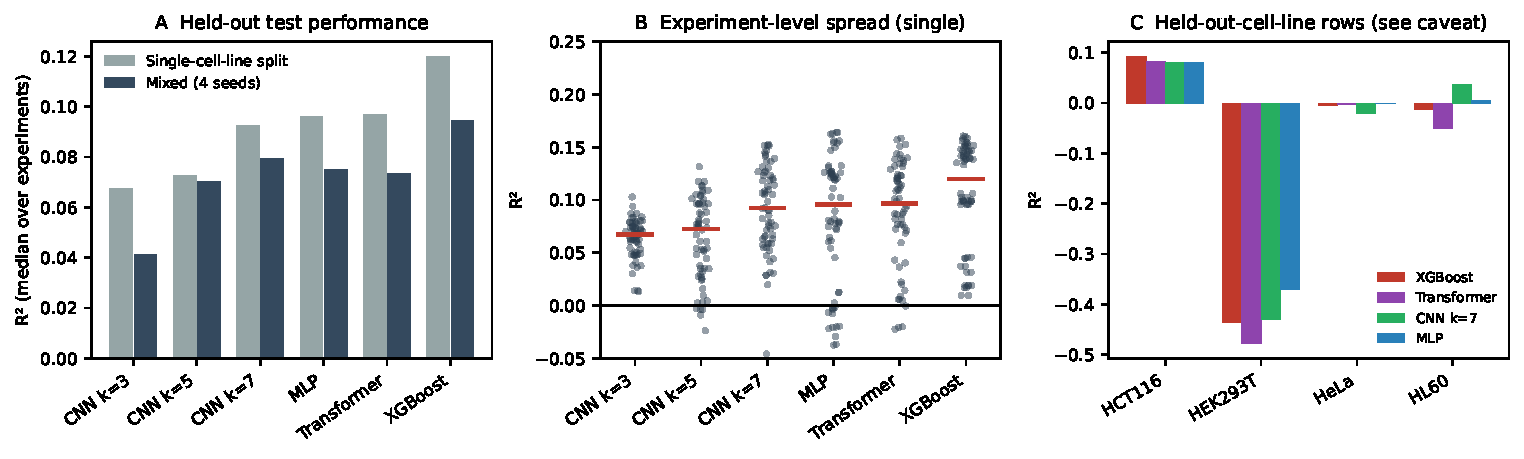
\includegraphics[width=\textwidth]{figures/fig2_prediction.pdf}
\caption{留出测试集预测性能（每配置 64 次运行）。\textbf{(A)} \emph{single}、\emph{mixed} 与 \emph{all}（真实 LOCO）三种划分下各模型配置的 $R^{2}$ 中位数；LOCO 分支整体落在 0 附近或以下。\textbf{(B)} \emph{single} 划分下逐次运行的 $R^{2}$ 分布（散点为单次实验，红线为中位数），可见 Linear Regression 的发散运行。\textbf{(C)} 按留出细胞系展开的 LOCO 行，显示极端的细胞系间异质性（HEK293T 最低）。}
\label{fig:prediction}
\end{figure}

\subsection{泄漏整改前后的对照（E1 方法学）}
\label{sec:res-leakage}

\textbf{问题与方法.} 项目早期批次（\texttt{batch\_20260909\_full}）采用按记录随机划分，且 LOCO 分支未剔除留出系同源序列。为量化该问题的影响，我们比较整改前后两个批次的同一批统计量（两批使用相同的数据、模型配置与环境组合，仅划分策略不同；旧批次不进入本文任何结论）。

\textbf{观察.} 整改后 \emph{mixed} 划分的中位 $R^{2}$ 由 0.1184 降至 0.0734，\emph{all}（LOCO）由 $+0.0362$ 降至 $-0.0083$，而 \emph{single} 划分基本不变（0.0704 $\rightarrow$ 0.0808）。

\textbf{解释（假设）.} 三种划分的差异化变化说明：受影响的正是"训练与测试之间存在同源序列"的情形。\emph{single} 划分在单细胞系内部进行，序列唯一（该系内无重复序列），因此不受影响；\emph{mixed} 与 LOCO 涉及跨细胞系合并，此前同一 sgRNA 序列可同时进入训练与测试两侧，模型在测试集上部分"记忆"了已见序列，从而系统性高估跨细胞系性能。

\textbf{边界.} 本文不主张"旧批次结果全部无效"：在无同源重复的 \emph{single} 划分上两批结论一致。同样也不主张"模型完全没有跨细胞系泛化能力"：LOCO 中位 $R^{2}$ 接近 0 而非显著为负，且 HCT116 作为留出系时仍为正（$+0.043$）。准确的陈述是：\textbf{在排除同源序列污染后，跨细胞系泛化性能从"弱正"变为"与均值基线无法区分"}。

\subsection{环境增量信息：四个因子均未达到预设效应门槛（E1）}
\label{sec:res-environment}

\textbf{问题与方法.} 表观遗传环境是否在序列信息之外提供额外\emph{预测}信息？我们以 sequence-only 为基线，对 16 个环境组合的全部 lattice 边计算配对 $\Delta R^{2}$，并用逐样本配对 bootstrap、符号翻转置换检验与区组析因方差分析三种互补方式评估。

\textbf{观察 1（效应量级低于预设门槛）.} 四个因子的跨模型等权平均主效应为：CTCF $+0.0003$（95\% 区间 $-0.0035$--$0.0038$）、DNase $+0.0013$（$-0.0013$--$0.0043$）、H3K4me3 $-0.0007$（$-0.0033$--$0.0018$）、RRBS $-0.0015$（$-0.0040$--$0.0010$）。\textbf{四个因子的区间全部跨 0，且 $|\overline{\Delta R^{2}}|$ 为 $3.2\times10^{-4}$ 至 $1.5\times10^{-3}$，比预设的最小绝对增益门 $0.01$ 低 1--2 个数量级}（表~\ref{tab:environment}、图~\ref{fig:environment}A--B）。

\textbf{观察 2（边级与置换检验的一致性有限）.} 在 1\,978 条可检验 lattice 边上，逐样本配对 bootstrap 的 95\% 置信区间有 640 条不跨 0（CTCF 163/496、DNase 155/492、H3K4me3 168/494、RRBS 154/496）；四个因子的 \emph{Minimal Edge-level FDR across Tested Contexts} 均为 0.0070，但其为\emph{跨上下文取最小}的 existence-oriented 证据（FWER 上界 0.427--0.441），不足以提升因子等级。

\textbf{观察 3（区组析因方差分析未检出任何显著效应）.} 以 $R^{2}$ 为响应、四个环境因子为二水平因子、模型/细胞系/划分为区组的 Type-II 析因方差分析给出四个主效应 $p=0.975$--$0.9996$（CTCF 0.9892、DNase 0.9996、H3K4me3 0.9753、RRBS 0.9867），六个成对交互 $p=0.58$--$0.97$（图~\ref{fig:environment}D）。

\textbf{解释（假设）与边界.} 综合三种方法，本数据集\textbf{没有}提供支持"这四个环境因子具有达到预设门槛的独立增量预测贡献"的证据。这一结论的准确含义是\emph{未检出}，而不是\emph{无作用}：$\Delta R^{2}$ 度量的是在已有序列模型基础上的增量预测价值，环境信息可能与序列特征冗余、可能受限于二值化编码的分辨率\citep{Klemm2019NatRevGenet}，四个通道也不足以代表完整 cell state；此外若干细胞系--通道组合近乎常数，这会直接压缩可检测的效应上限。值得注意的是，已有研究报告在 sgRNA 活性预测中加入 DNase 可及性轨道后\textbf{并未}提升预测性能\citep{Wang2019NatCommun}。因此本结果为"在通用多细胞系设定下未检出"。统计可检测性与生物学相关性是两件事，本文只报告前者。

\begin{figure}[htbp]
\centering
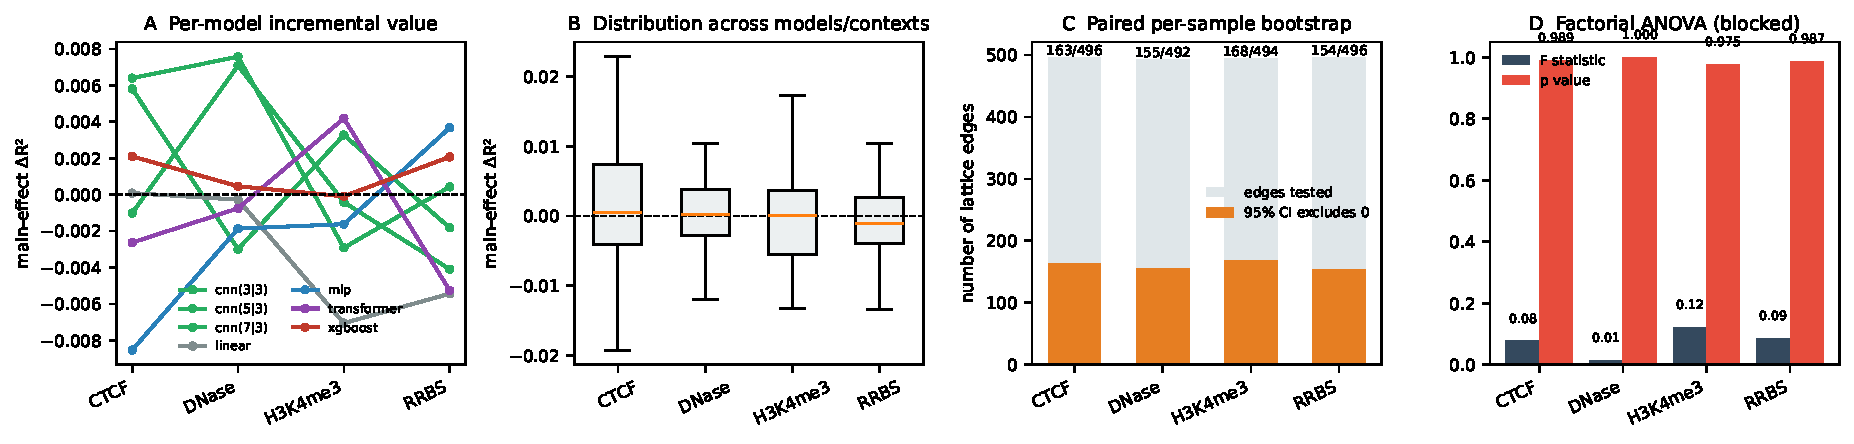
\includegraphics[width=\textwidth]{figures/fig3_environment.pdf}
\caption{环境因素的增量预测贡献与统计证据。\textbf{(A)} 各模型配置对四个环境因子的主效应 $\Delta R^{2}$（排除发散行）。\textbf{(B)} 主效应跨模型/上下文的分布。\textbf{(C)} 逐样本配对 bootstrap 中 95\% 置信区间不跨 0 的 lattice 边数量（分母为可检验边数）。\textbf{(D)} 区组析因方差分析的 $p$ 值；四个主效应与全部交互项均未达到 $p<0.05$。所有效应量级均小于 0.01。}
\label{fig:environment}
\end{figure}

\begin{table}[htbp]
\centering
\footnotesize
\caption{Environmental factors: cross-model incremental predictive value (mean main-effect ΔR² over models after excluding numerically diverged rows, |ΔR²| > 10), model-level bootstrap interval (n = 7 model configurations), paired per-sample edge bootstrap (CI excluding zero), permutation-based FDR, blocked factorial ANOVA and cell-line context label. Effect gate = $|$model-equal-weight mean $\Delta R^{2}| \ge 0.01$; min\_edge\_FDR = Minimal Edge-level FDR across Tested Contexts (existence-oriented, extremum selection, not a factor-level FDR); n\_contexts = de-duplicated tested contexts; mlevel\_bootstrap = Model-Level Bootstrap Interval (n = 7 model configurations).}
\label{tab:environment}
\resizebox{\textwidth}{!}{%
\begin{tabular}{lrrrrrrrrrrrrrrrr}
\toprule
factor & mean\_dR2 & median\_dR2 & effect\_gate & n\_models & direction\_conflict & min\_edge\_FDR & n\_contexts & selected\_context & fwer\_upper\_bound & concordance & mlevel\_bootstrap & ci\_excludes\_zero & anova\_F & anova\_p & cell\_line\_context & tier \\
\midrule
CTCF & 0.0003 & 0.0001 & fail & 7 & yes & 0.0070 & 63 & all/hl60/linear & 0.4406 & 0.5714 & [-0.0035, 0.0038] & False & 0.0773 & 0.9892 & Context-conflicting & Inconclusive \\
DNASE & 0.0013 & -0.0003 & fail & 7 & yes & 0.0070 & 61 & all/hl60/linear & 0.4266 & 0.5714 & [-0.0013, 0.0043] & False & 0.0142 & 0.9996 & Uncertain & Inconclusive \\
H3K4ME3 & -0.0007 & -0.0004 & fail & 7 & yes & 0.0070 & 62 & all/hl60/linear & 0.4336 & 0.7143 & [-0.0033, 0.0018] & False & 0.1204 & 0.9753 & Context-conflicting & Inconclusive \\
RRBS & -0.0015 & -0.0018 & fail & 7 & yes & 0.0070 & 63 & all/hl60/linear & 0.4406 & 0.5714 & [-0.0040, 0.0010] & False & 0.0863 & 0.9867 & Uncertain & Inconclusive \\
\bottomrule
\end{tabular}
}
\end{table}


\subsection{多模型序列归因指向 PAM 邻近位置（E3）}
\label{sec:res-sequence}

\textbf{问题与方法（RQ2 的第一半）.} 模型归因是否指向可重复的序列位置，且这种指向是否跨模型类一致？我们比较五类模型的主归因方法（线性系数、TreeSHAP、MLP-IG、CNN-IG、注意力）在 23 个位置上的归一化归因分布，并分别在\textbf{单碱基位置}与\textbf{粗粒度区域}两个层级汇总。

\textbf{观察 1（单模型峰值：4/5 个模型类落在 PAM 邻近窗口）.} 每个模型类的跨上下文平均归因谱的峰值位置为：XGBoost 第 18 位（0.1345）、MLP 第 18 位（0.0857）、Transformer 第 19 位（0.1045）、CNN 第 20 位（0.0529），即\textbf{四个非模型类的峰值都落在 PAM 邻近窗口 17--20 内}；唯一的例外是 Linear Regression，其峰值在第 1 位（0.1977）——线性模型在剔除 \texttt{\_T} 参照列后，首位碱基承担了基线效应。

\textbf{观察 2（跨模型平均谱：位置 1 与位置 18 之争取决于是否纳入 Linear）.} 把五个模型类等权平均后，谱峰位于\textbf{第 1 位（0.0864）}，其后为第 18 位（0.0799）、第 20 位（0.0708）、第 19 位（0.0637）；该首位峰值完全由 Linear 贡献。\textbf{剔除 Linear 后，四个模型的平均谱峰值为第 18 位（0.0878）}，其后为第 20 位（0.0764）、第 19 位（0.0669）（表~\ref{tab:attribution-position}）。本文因此不写"跨模型平均谱峰值即为第 18 位"这一概括，而是并列两种口径——这是"保留模型间分歧而非平均掉"的具体执行。

\textbf{观察 3（逐上下文的峰值落点比例）.} 在 \emph{single} 划分的 64 个（细胞系 $\times$ 环境）上下文下，统计各模型类的归因峰值是否落在 17--20 窗口：\textbf{XGBoost 100.0\%（64/64）、CNN 96.9\%（62/64）、MLP 90.6\%（58/64）、Transformer 65.6\%（42/64）、Linear 21.9\%（14/64）}。众数位置分别为第 18 位（XGBoost、MLP）、第 20 位（CNN）、第 19 位（Transformer）、第 1 位（Linear）。

\textbf{观察 4（区域层级：仅两个模型类的最高区域为 PAM 邻近区）.} 按四个粗粒度区域汇总（对细胞系与上下文取平均）后，XGBoost（PAM 邻近区 0.327）与 Transformer（0.325）的最高归因区域确为 PAM 邻近种子区（17--20）；但 \textbf{CNN（0.344）与 MLP（0.336）的最高区域为种子核心区（9--16）}，而 Linear Regression 的最高区域为 PAM 远端区（0.416）（图~\ref{fig:sequence}B）。即\textbf{只有 2/5 个模型类的最高区域是 PAM 邻近区}。跨模型位置谱的平均两两 Spearman 相关系数为 0.34（80 个上下文，范围 0.03--0.56），top-3 位置重叠率 0.42。

\textbf{统计证据.} 观察 1--4 均为归因幅值的描述性汇总。\textbf{attribution 幅值不构成统计显著性证据}；本文不报告归因的 $p$ 值，也不把 SNR 当作检验统计量（\S\ref{sec:methods}）。

% 本文件由 analysis/reporting/paper_rewrite/build_rewrite_tables.py 自动生成。
% 请勿手工编辑；数字来源见文件头注释与 results/paper_rewrite/authoritative_numbers.json。
\begin{table}[htbp]
\centering
\footnotesize
\caption{位置层级归因（E3；测试集口径与 \emph{single} 划分）。上：各模型类跨上下文平均归因谱的峰值位置与峰值，以及逐上下文峰值落在 PAM 邻近窗口（17--20）的比例（分母为 64 个 细胞系 $\times$ 环境 上下文）。下：等权平均谱的前五位。\textbf{五模型平均谱的峰值是第 1 位而非第 18 位}，该峰值完全由 Linear 贡献；剔除 Linear 后峰值才是第 18 位。本文并列两种口径而不取其一。归因幅值仅表示模型依赖强度，不构成统计显著性证据。}
\label{tab:attribution-position}
\begin{tabular}{lrrrr}
\toprule
model class & 峰值位置 & 峰值 & 峰值 $\in[17,20]$ 的比例 & 众数位置 \\
\midrule
Linear & 1 & 0.1977 & 21.9\% (14/64) & 1 \\
XGBoost & 18 & 0.1345 & 100.0\% (64/64) & 18 \\
Transformer & 19 & 0.1045 & 65.6\% (42/64) & 19 \\
MLP & 18 & 0.0857 & 90.6\% (58/64) & 18 \\
CNN & 20 & 0.0529 & 96.9\% (62/64) & 20 \\
\midrule
\multicolumn{5}{l}{\textit{等权平均谱前五位}} \\
五模型（含 Linear） & \multicolumn{4}{l}{1 (0.0864) $>$ 18 (0.0799) $>$ 20 (0.0708) $>$ 19 (0.0637) $>$ 21 (0.0461)} \\
\midrule
四模型（剔除 Linear） & \multicolumn{4}{l}{18 (0.0878) $>$ 20 (0.0764) $>$ 19 (0.0669) $>$ 1 (0.0586) $>$ 21 (0.0519)} \\
\bottomrule
\end{tabular}
\end{table}


\textbf{解释（假设）与边界.} 支持"PAM 邻近区域（尤其第 18/20 位）是与编辑效率最相关的序列位置"这一表述的证据在\textbf{位置层级较强}：四个非模型类（XGBoost、CNN、MLP、Transformer）的逐上下文峰值落在 17--20 窗口的比例为 65.6\%--100\%，且它们的单模型平均谱峰值都在该窗口内。但该表述有三个必须同时声明的边界：其一，\textbf{Linear 完全不符合}（21.9\%，峰值在第 1 位），因此不能说"五类模型一致"；其二，把 Linear 纳入平均后，\textbf{跨模型平均谱峰值是第 1 位而非第 18 位}；其三，在\textbf{区域层级仅为 2/5}。本文因此采用如下表述：\emph{四个非模型类的位置归因峰值高度集中于 PAM 邻近窗口，线性模型则集中于首位与 PAM 区；两种口径下第 18 位都位列前二，但并非在所有口径下都是第一。} 这一分歧被\textbf{保留而非平均掉}，并作为 \S\ref{sec:res-external} 选择第 18 位做外部验证的动机之一——但必须强调：\textbf{E3 自身不能说明该位置是否真的重要，它只说明模型依赖该位置}。

\begin{figure}[htbp]
\centering
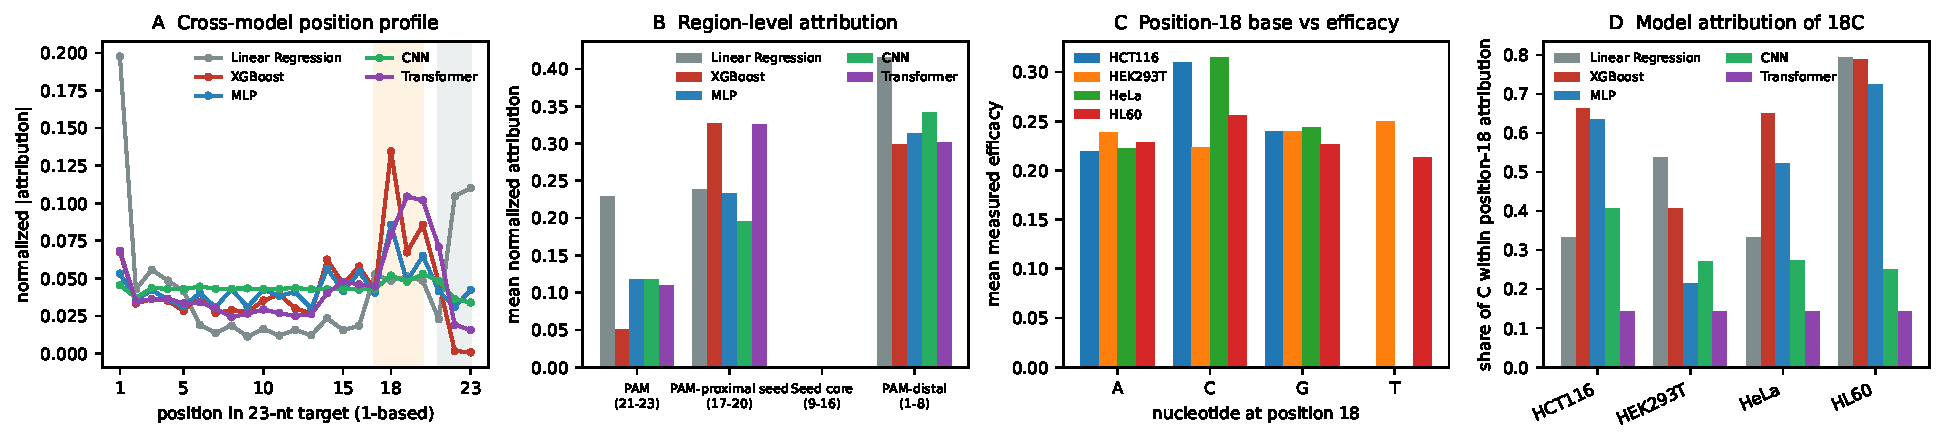
\includegraphics[width=\textwidth]{figures/fig4_sequence_attribution.pdf}
\caption{跨模型序列归因。\textbf{(A)} 五类模型在 23 个位置上的归一化归因谱（阴影为 PAM 邻近种子区 17--20 与 PAM 21--23）。\textbf{(B)} 四个序列区域的平均归一化归因（按模型）；仅 XGBoost 与 Transformer 的最高区域为 PAM 邻近区（2/5）。归因幅值仅表示模型依赖强度，不构成统计显著性证据；不同模型的 importance 在模型内归一化，绝对值不可跨模型类直接比较。}
\label{fig:sequence}
\end{figure}

\subsection{多尺度 CNN：更宽的局部感受野带来小幅但可复现的提升（E1 $+$ E3）}
\label{sec:res-kernel}

\textbf{问题与方法.} 序列卷积核大小（感受野）是否影响预测与解释？我们在 192 组严格配对的实验（同一划分、细胞系、环境组合与种子，仅卷积核不同）中比较 $R^{2}$，并比较三个核配置的归因谱与候选模式长度。

\textbf{观察 1（提升方向一致但幅度有限）.} 配对差分为：$k=5$ 相对 $k=3$ 提高 $+0.0046$（95\% bootstrap 区间 $-0.0029$--$+0.0116$，66.2\% 配对为正，\textbf{区间跨 0}）；$k=7$ 相对 $k=3$ 提高 $+0.0169$（$+0.0077$--$+0.0257$，79.7\% 为正）；$k=7$ 相对 $k=5$ 提高 $+0.0123$（$+0.0070$--$+0.0175$，70.8\% 为正）（表~\ref{tab:kernel}、图~\ref{fig:kernel}A）。

\textbf{观察 2（解释随之改变）.} 区域平均归因显示，感受野增大使归因向 PAM 邻近区与 PAM 区集中，而 PAM 远端区下降（图~\ref{fig:kernel}C）。这直接说明\textbf{归因对模型超参数敏感}。

\textbf{观察 3（模式长度不随核大小改变）.} 三个核配置提取的候选模式长度中位数均为 4\,nt（分布 4--11），说明\textbf{卷积核大小是模型感受野参数，不能等同于候选模式长度}。

\textbf{解释（假设）与边界.} 结果支持一个模型层面的谨慎解释：在本案例数据中，更宽的局部感受野能更好地捕获 PAM 邻近上下文的依赖关系，从而带来小幅但方向一致的预测提升。该结论\emph{限于 E1 与 E3}，不能推断"更宽的序列上下文具有生物学因果必要性"。

\begin{figure}[htbp]
\centering
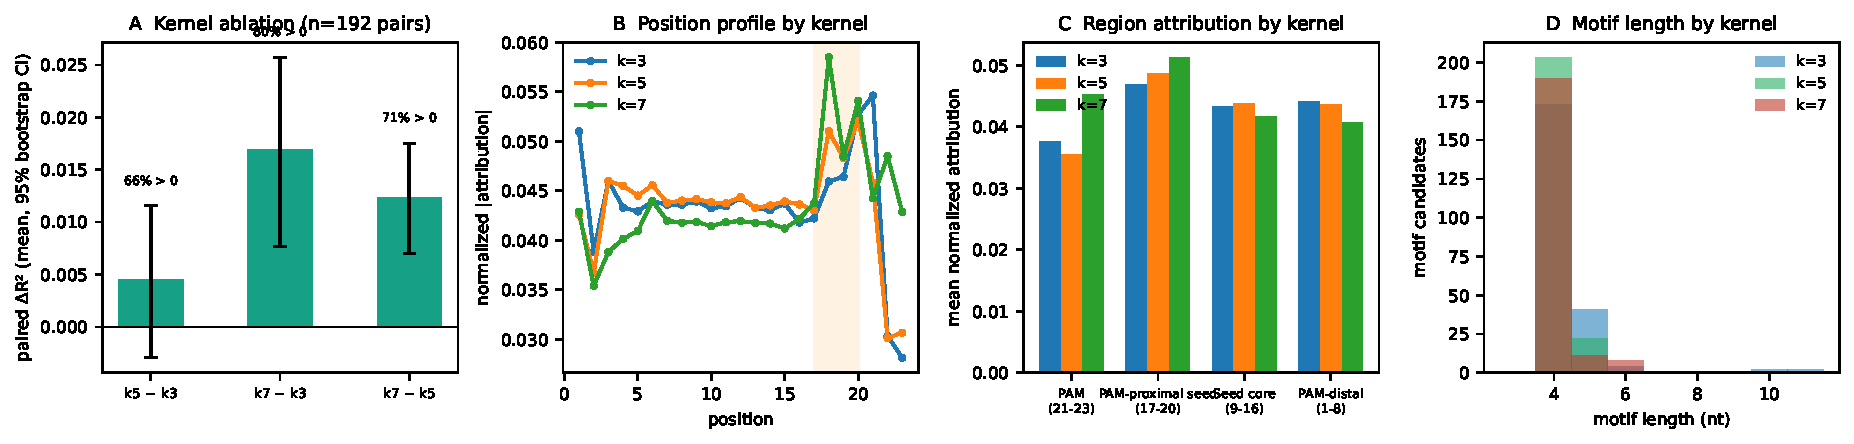
\includegraphics[width=\textwidth]{figures/fig5_kernel.pdf}
\caption{CNN 感受野（多尺度局部序列上下文）分析。\textbf{(A)} 192 组配对实验的 $\Delta R^{2}$（均值与 95\% bootstrap 区间），标注配对中为正的比例与区间是否跨 0。\textbf{(B)} 三个核配置的位置归因谱。\textbf{(C)} 区域平均归因随核大小的变化。\textbf{(D)} 三配置提取的候选模式长度分布（中位数均为 4\,nt）。}
\label{fig:kernel}
\end{figure}

\begin{table}[htbp]
\centering
\footnotesize
\caption{CNN receptive-field (kernel size) ablation. Paired differences of held-out R² over 192 matched experiment pairs (same split, cell line, environment and seed); CI is a percentile bootstrap over pairs.}
\label{tab:kernel}
\begin{tabular}{lrrrrrr}
\toprule
comparison & n\_pairs & mean\_dR2 & ci\_low & ci\_high & pct\_positive & excludes\_zero \\
\midrule
k5 $-$ k3 & 192 & 0.0046 & -0.0029 & 0.0116 & 0.6615 & False \\
k7 $-$ k3 & 192 & 0.0169 & 0.0077 & 0.0257 & 0.7969 & True \\
k7 $-$ k5 & 192 & 0.0123 & 0.0070 & 0.0175 & 0.7083 & True \\
\bottomrule
\end{tabular}
\end{table}


\subsection{候选序列模式及其统计支持（E3 $+$ 富集检验）}
\label{sec:res-motifs}

\textbf{问题与方法.} 归因能否进一步形成具有支持度、方向与统计检验的候选序列模式？我们按 \S\ref{sec:methods} 流程从 CNN IG/ISM 归因中提取 seqlet 并聚类，随后进行共识构建、支持度筛选与富集检验。

\textbf{观察.} 最终得到 \textbf{656 个候选模式}（标签反映跨核与跨细胞系复现性），长度以 4\,nt 为主；位置分布高度集中于 PAM 邻近区。富集检验（前景为效率上三分位序列，背景为全部可用序列）共 656 次，其中 \textbf{65 个通过 BH-FDR $<0.05$（9.9\%）}（表~\ref{tab:motifs}）。

\textbf{统计证据.} 富集检验提供的是"该模式在高效序列中更常见"的统计支持；由于多数候选模式与 PAM/种子区重叠，其统计支持部分来自该区域的整体重要性，未必构成独立的模式语法。

\textbf{解释（假设）与边界.} 三项限制尤须强调：其一，候选模式目前\textbf{仅具计算证据}，跨模型比较仅限 CNN 三个核配置（缺少 Transformer IG 产物），因此不能宣称"跨模型收敛的生物学 motif"；其二，富集结果目前多在单一细胞系（HeLa）中达到显著，属 context-dependent 候选；其三，通过 FDR 的 65 个模式须视为\emph{待实验验证的候选序列模式}，而不是功能性 motif。

\begin{table}[htbp]
\centering
\footnotesize
\caption{Representative motif candidates discovered from CNN attribution. Support counts are seqlet instances; enrichment and FDR come from the Fisher exact test against the all-eligible-sequence background (BH-FDR within the motif\_enrichment family). Effect direction is the carrier-vs-background measured-efficiency contrast, not a causal effect.}
\label{tab:motifs}
\resizebox{\textwidth}{!}{%
\begin{tabular}{lrrrrrrrrrrrr}
\toprule
motif\_id & human\_pattern & iupac & regex & length & support\_count & sample\_support & cellline\_support & effect\_direction & mean\_effect & enrichment & FDR & evidence\_strength \\
\midrule
motif\_cnn33\_hela\_sequence\_cnn\_ig\_001 & CTGG & CTGG & CTGG & 4 & 1273 & 1273 & 1 & - & -0.046 & 0.870 & 1.000 & Moderate motif evidence \\
motif\_cnn33\_hela\_sequence\_cnn\_ig\_012 & CAGG & CAGG & CAGG & 4 & 1083 & 1083 & 1 & - & -0.030 & 0.934 & 1.000 & Moderate motif evidence \\
motif\_cnn33\_hela\_sequence\_cnn\_ig\_025 & GAGG & GAGG & GAGG & 4 & 899 & 899 & 1 & + & 0.012 & 1.081 & 0.031 & Strong motif evidence \\
motif\_cnn33\_hela\_all\_cnn\_ig\_032 & AAGG & AAGG & AAGG & 4 & 890 & 890 & 1 & - & -0.010 & 0.983 & 1.000 & Moderate motif evidence \\
motif\_cnn33\_hela\_sequence\_cnn\_ig\_044 & ATGG & ATGG & ATGG & 4 & 789 & 789 & 1 & + & 0.011 & 1.050 & 0.259 & Moderate motif evidence \\
motif\_cnn33\_hela\_sequence\_cnn\_ig\_057 & GTGG & GTGG & GTGG & 4 & 740 & 740 & 1 & + & 0.017 & 1.030 & 0.466 & Moderate motif evidence \\
motif\_cnn33\_hela\_sequence\_cnn\_ig\_086 & AGGG & AGGG & AGGG & 4 & 610 & 610 & 1 & + & 0.028 & 1.068 & 0.206 & Moderate motif evidence \\
motif\_cnn33\_hela\_sequence\_cnn\_ism\_119 & GCTG & GCTG & GCTG & 4 & 482 & 482 & 1 & - & -0.061 & 0.872 & 1.000 & Model-specific motif \\
motif\_cnn53\_hela\_all\_cnn\_ig\_120 & GCTGG & GCTGG & GCTGG & 5 & 482 & 482 & 1 & - & -0.061 & 0.801 & 1.000 & Model-specific motif \\
motif\_cnn33\_hela\_sequence\_cnn\_ig\_147 & GGGG & GGGG & GGGG & 4 & 435 & 435 & 1 & + & 0.060 & 1.353 & 0.000 & Exploratory motif \\
\bottomrule
\end{tabular}
}
\end{table}


\subsection{外部模型验证：独立第三方模型确认第 18 位扰动方向（E4，外部验证）}
\label{sec:res-external}

\textbf{问题与方法（RQ2 的第二半）.} \S\ref{sec:res-sequence} 的结论完全建立在本文自己的模型族上：五类模型可能\textbf{共同依赖了同一份数据中的同一混杂结构}。因此我们引入独立第三方模型 CRISPRon（不同训练数据、不同输入编码、不同输出尺度；\S\ref{sec:methods-external}），把 E3 指认的位置转化为一个最小扰动，检验\textbf{两个独立系统对同一扰动的方向判断是否一致}。

\textbf{观察 1（预登记的选择规则）.} 我们从 DeepCRISPR \emph{single} 划分的\textbf{测试集}中，按预先写死的规则（独立于任何突变侧信息，脚本内以断言强制）选出 8 条第 18 位为 C 的代表性 WT 序列，覆盖 low/medium/high 三个效率区间与 4 个细胞系（表~\ref{tab:externalvalidation}）。选择规则在扰动之前固定，因此"下降多少"不可能影响"选了谁"。

\textbf{观察 2（外部模型的扰动响应与本文模型族方向一致）.} 每条 WT 只改第 18 位一个碱基（C$\rightarrow$A），其余 22\,nt 与全部侧翼逐位不变（逐条 QC 通过：仅目标位点改变、PAM 未变、侧翼一致、方向保持、WT 与突变体各恰好命中 1 个预期靶点）。结果显示：

\begin{itemize}
\item \textbf{CRISPRon 侧：8 条中有 7 条给出负向变化}（方向一致率 $0.875$），$\Delta$ 均值为 $-12.43$、中位 $-13.82$、范围 $-27.17$ 至 $+9.16$；
\item \textbf{跨模型方向一致性为 7/8}：本文 7 个模型的符号化 ISM 预测变化（$\Delta_{\text{ours}}$）与 CRISPRon 的 $\Delta$ 在 7 条序列上同号；
\item 两个系统的\textbf{变化幅度也正相关}：Pearson $r=0.629$，Spearman $\rho=0.476$（$n=8$）；
\item 唯一分歧为 \textbf{WT08}（本文模型 $\Delta_{\text{ours}}=-0.021$，CRISPRon $\Delta=+9.16$）。\textbf{该序列被保留在全部统计中，而非剔除为异常值}。
\end{itemize}

\textbf{观察 3（外部验证的独立性是可核查的）.} CRISPRon 的安装与运行经过官方黄金测试：\texttt{bin/test.sh} 输出 \texttt{TEST ok}，且生成的中间文件与官方 \texttt{test/outdir.original/} 中的对应文件逐字节相同（SHA-256 相等）。CRISPRon 会在正负两条链上扫描 30-mer，因此额外靶点被显式计数（本批 3 条记录出现额外命中，均记录在案）。

\textbf{统计证据.} 方向一致性为 $7/8$，幅度相关的 $n=8$。样本量小，本文\textbf{不}对 $r$ 或 $\rho$ 做显著性检验，也不把 $0.875$ 解读为总体比例估计；报告的是这 8 个预登记实例上的实际一致性计数。

\textbf{解释（假设）与边界.} 该结果把"第 18 位对模型预测有实质影响"这一陈述从\emph{单一模型族内的观察}提升为\emph{跨独立系统的可复现观察}。但必须严格限定：这仍然是\textbf{模型行为层面}的证据（E4）。\textbf{两个模型系统方向一致，可以说明它们捕捉到了同一统计结构，不能说明该结构对应真实的编辑效率变化。} 尤其注意：WT08 的分歧说明这一致性并非普遍成立，本文不隐去它。

\begin{figure}[htbp]
\centering
\begin{tabular}{cc}
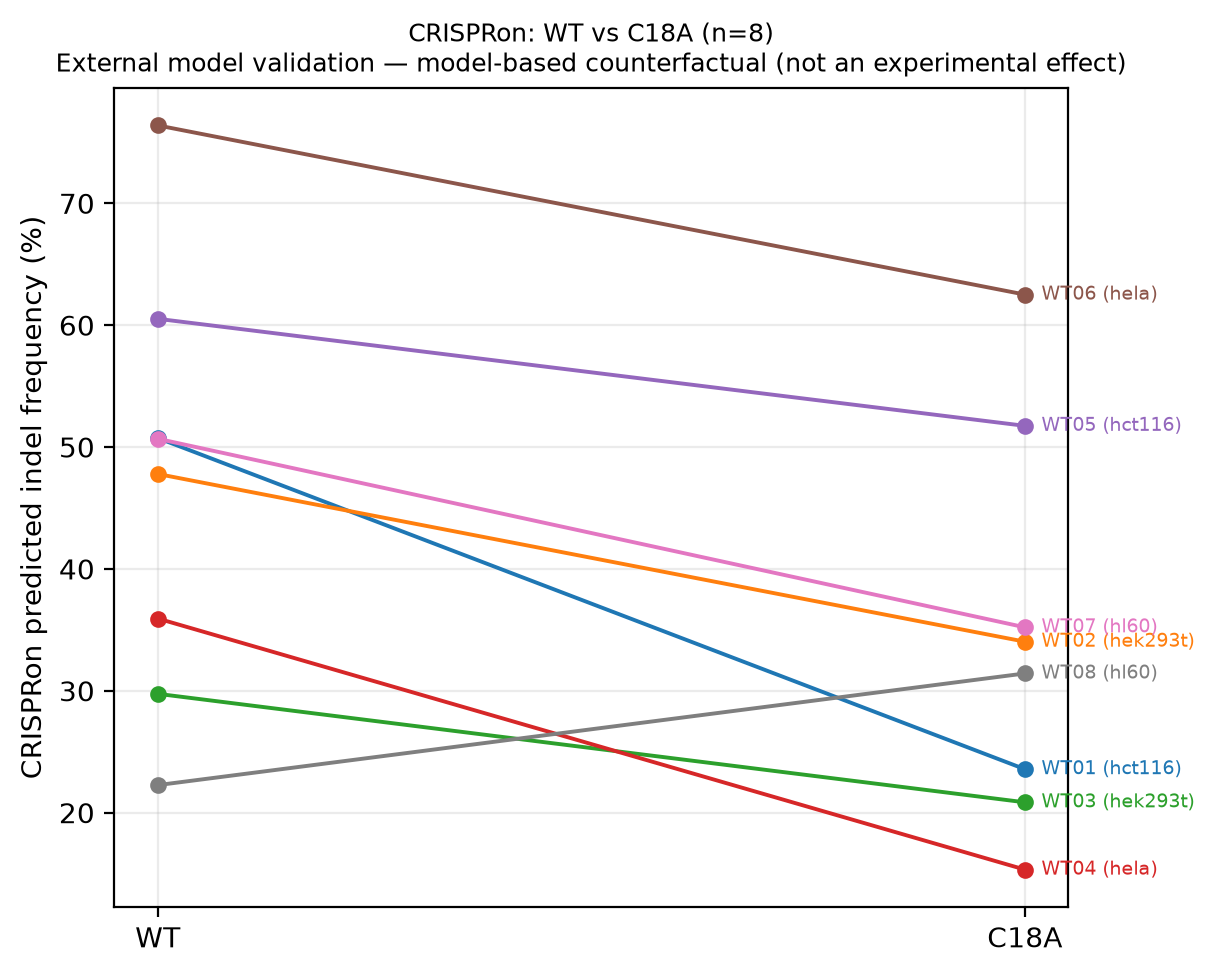
\includegraphics[width=0.47\textwidth]{figures/fig_ext_a_wt_vs_c18a.png} &
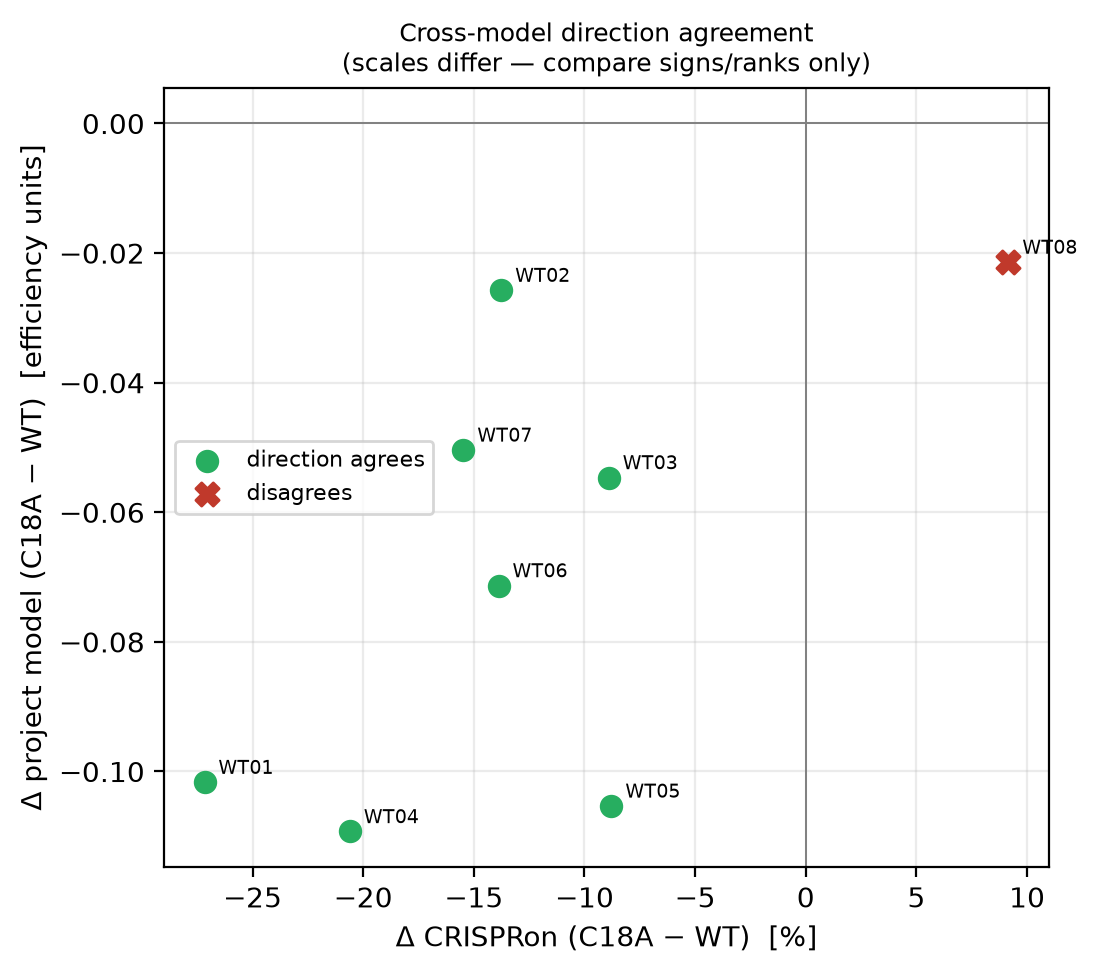
\includegraphics[width=0.47\textwidth]{figures/fig_ext_b_ours_vs_crispron.png} \\[2pt]
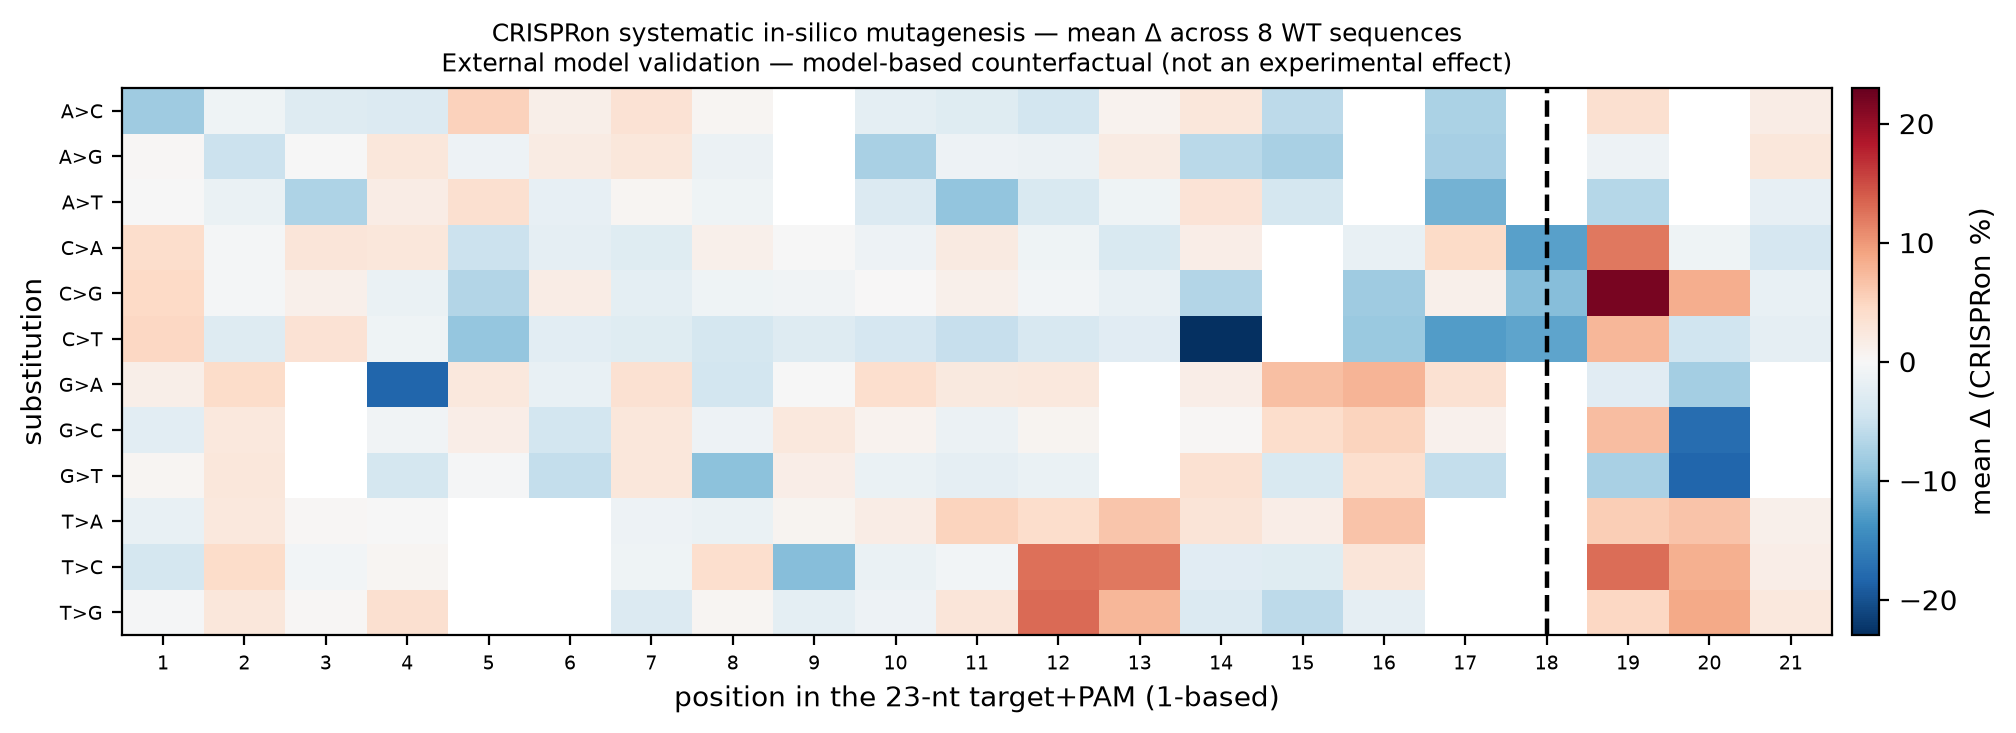
\includegraphics[width=0.47\textwidth]{figures/fig_ext_c_position_heatmap.png} &
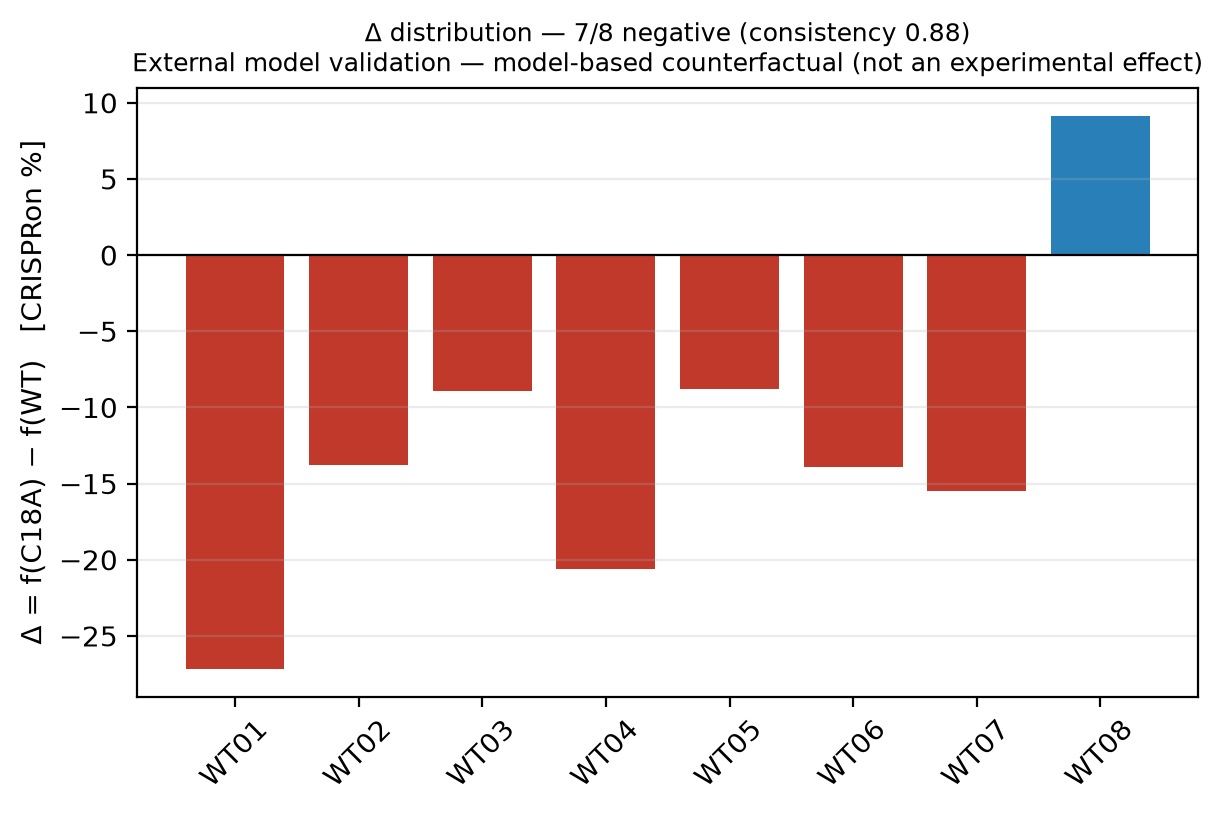
\includegraphics[width=0.47\textwidth]{figures/fig_ext_d_delta_distribution.png}
\end{tabular}
\caption{外部模型验证（E4）。左上：8 条预登记 WT 序列在 C$\rightarrow$A 前后由 CRISPRon 给出的评分配对变化。右上：本文 7 个模型的 $\Delta_{\text{ours}}$ 与 CRISPRon 的 $\Delta$ 的对应关系（$r=0.629$，$\rho=0.476$，$n=8$）；对角线上方/下方分别表示方向一致/不一致，WT08 为唯一分歧点。左下：全部 552 条单碱基替换的 $\Delta$ 矩阵（按位置），可见第 18 位列的颜色最深。右下：$\Delta$ 的分布。}
\label{fig:external}
\end{figure}

% 本文件由 analysis/reporting/paper_rewrite/build_rewrite_tables.py 自动生成。
% 请勿手工编辑；数字来源见文件头注释与 results/paper_rewrite/authoritative_numbers.json。
\begin{table}[htbp]
\centering
\footnotesize
\caption{外部模型验证：独立第三方模型 CRISPRon 对第 18 位 C$\rightarrow$A 反事实扰动的响应。8 条野生型（WT）序列按预先登记规则从 DeepCRISPR 测试集选出（第 18 位为 C），扰动仅改变第 18 位一个碱基，其余 22\,nt 与全部侧翼完全不变（逐条 QC 通过）。$\Delta_{\text{CRISPRon}}$ 为 CRISPRon 复合评分（0--100）；$\Delta_{\text{ours}}$ 为本文 7 个模型基于符号化 in-silico 突变的预测变化均值 $\pm$ 标准差（归一化效率尺度）。\textbf{两个模型族的扰动响应在 8 条序列中的 7 条上方向一致}（Pearson $r=0.629$，Spearman $\rho=0.476$，$n=8$）；唯一分歧为 WT08，该结果保留而非剔除。}
\label{tab:externalvalidation}
\begin{tabular}{llrrrrrc}
\toprule
sample & cell line & 实测效率 & CRISPRon WT & CRISPRon C18A & $\Delta_{\text{CRISPRon}}$ & $\Delta_{\text{ours}}$ & 方向一致 \\
\midrule
WT01 & hct116 & 0.110 & 50.74 & 23.57 & -27.17 & -0.102 $\pm$ 0.038 & 是 \\
WT02 & hek293t & 0.144 & 47.79 & 34.03 & -13.76 & -0.026 $\pm$ 0.025 & 是 \\
WT03 & hek293t & 0.214 & 29.75 & 20.85 & -8.90 & -0.055 $\pm$ 0.032 & 是 \\
WT04 & hela & 0.267 & 35.93 & 15.33 & -20.60 & -0.109 $\pm$ 0.053 & 是 \\
WT05 & hct116 & 0.537 & 60.52 & 51.74 & -8.78 & -0.105 $\pm$ 0.073 & 是 \\
WT06 & hela & 0.503 & 76.39 & 62.51 & -13.88 & -0.071 $\pm$ 0.023 & 是 \\
WT07 & hl60 & 0.344 & 50.68 & 35.21 & -15.47 & -0.050 $\pm$ 0.027 & 是 \\
WT08 & hl60 & 0.187 & 22.26 & 31.42 & +9.16 & -0.021 $\pm$ 0.028 & \textbf{否} \\
\midrule
\multicolumn{8}{l}{CRISPRon 侧：7/8 条 $\Delta<0$，方向一致率 0.875，$\Delta$ 均值 -12.43（中位 -13.82，范围 -27.17 至 +9.16）} \\
\bottomrule
\end{tabular}
\end{table}


\subsection{反事实扰动：饱和突变独立地把第 18 位排在首位（E4）}
\label{sec:res-counterfactual}

\textbf{问题与方法.} \S\ref{sec:res-external} 检验的是"预先指定的位置"。为排除"我们恰好挑了一个看起来重要的位置"这一可能，我们做一个\textbf{不预先指定位置}的穷举检验：对 8 条 WT 的 23 个位点、每个位点的全部 3 种非野生型替换做饱和 in-silico 突变，用 CRISPRon 打分，再比较各位置的平均效应量级。

\textbf{观察 1（第 18 位在全部可比位置中排名第 1）.} 共产生 552 条替换记录（$8\times23\times3$），其中 48 条破坏 PAM 而无法被 CRISPRon 识别、被排除，剩 504 条计分。按平均 $|\Delta|$ 排序（表~\ref{tab:counterfactual}），前五位为第 18 位（12.86）$>$ 第 17 位（7.68）$>$ 第 20 位（7.18）$>$ 第 19 位（6.99）$>$ 第 16 位（5.36），\textbf{第 18 位排名 1/21}，且其量级约为第 2 名的 1.7 倍、最弱位置（第 21 位 2.13、第 2 位 2.60）的 5--6 倍。

\textbf{观察 2（该排名在逐序列层面也稳定）.} 在每条序列内部单独排序，第 18 位在 8 条序列中的 \textbf{7 条上排第 1}、1 条（WT08）上排第 2，排序中位数为 1.0，平均百分位 0.975。

\textbf{观察 3（C$\rightarrow$A 的方向与该位置的特异性）.} 第 18 位的 C$\rightarrow$A 平均变化为 $\mathbf{-12.425}$，而其余 19 个存在可用 C$\rightarrow$A 替换的位置平均仅 $+0.144$。即：在该位置上把 C 换成 A 会明显降低外部模型的预测评分，而同样操作放在别处则几乎没有影响。这与 \S\ref{sec:res-external} 的定向扰动结果自洽。

\textbf{统计证据.} 每条序列在第 18 位只有 1 个观测，样本量不足以做位置间显著性检验。本文\textbf{只报描述统计与排名}，不报告 $p$ 值。

\textbf{解释（假设）与边界.} 饱和实验的设计意义在于：它不是"我们想看第 18 位"，而是"穷举所有位置后第 18 位自己浮出来"。因此"第 18 位是外部模型最敏感的位置"这一陈述不再依赖于位置选择。但边界同样明确：这仍是\textbf{模型内部反事实}（E4）。一个对输入某位置高度敏感的模型，可能在真实细胞中完全错误。第 18 位是否真的影响编辑效率，只能由 E5（实验）回答。

% 本文件由 analysis/reporting/paper_rewrite/build_rewrite_tables.py 自动生成。
% 请勿手工编辑；数字来源见文件头注释与 results/paper_rewrite/authoritative_numbers.json。
\begin{table}[htbp]
\centering
\footnotesize
\caption{反事实扰动证据：在 8 条 WT 序列上对 23\,nt 靶序列的\textbf{全部单碱基替换}做饱和 in-silico 突变，并用外部模型 CRISPRon 评分。共 552 条替换记录（8 序列 $\times$ 23 位点 $\times$ 3 种替换），其中 48 条破坏 PAM 而无法被 CRISPRon 识别、被排除，剩 504 条计分；21 个位置可排名，20 个位置存在可用的 C$\rightarrow$A 替换。第 18 位的 C$\rightarrow$A 平均变化为 -12.425，而其余位置平均仅 +0.144；按平均 $|\Delta|$ 计，第 18 位（12.86）在 21 个位置中\textbf{排名第 1}。逐序列看，第 18 位在 8 条序列中的 7 条上排序第 1、1 条上第 2（排序中位数 1.0）。全部数值为\textbf{模型内部反事实}，不是实验测量。}
\label{tab:counterfactual}
\begin{tabular}{rrr@{\hspace{2em}}rrr@{\hspace{2em}}rrr}
\toprule
pos & 平均$|\Delta|$ & 排名 & pos & 平均$|\Delta|$ & 排名 & pos & 平均$|\Delta|$ & 排名 \\
\midrule
1 & 3.22 & 14 & 8 & 3.57 & 11 & 15 & 5.22 & 6 \\
2 & 2.60 & 20 & 9 & 3.32 & 13 & 16 & 5.36 & 5 \\
3 & 3.09 & 17 & 10 & 2.92 & 18 & 17 & 7.68 & 2 \\
4 & 3.19 & 15 & 11 & 3.83 & 9 & 18 & 12.86 & 1 \\
5 & 3.69 & 10 & 12 & 3.56 & 12 & 19 & 6.99 & 4 \\
6 & 3.18 & 16 & 13 & 4.54 & 7 & 20 & 7.18 & 3 \\
7 & 2.77 & 19 & 14 & 4.14 & 8 & 21 & 2.13 & 21 \\
\bottomrule
\end{tabular}
\end{table}


\subsection{观测性关联：第 18 位碱基效应及其细胞背景依赖（E2）}
\label{sec:res-association}

\textbf{问题与方法.} 上述 E3/E4 全部是模型产物。作为一条与模型\textbf{无关}的证据线，我们直接比较实测标签：按第 18 位碱基分组，计算各细胞系的平均归一化效率。

\textbf{观察 1（方向与模型一致，但幅度依赖细胞系）.} 第 18 位 C 减 A 的实测平均效率差为：HCT116 $+0.090$（C 0.309 vs A 0.219）、HeLa $+0.092$（0.315 vs 0.223）、HL60 $+0.027$（0.256 vs 0.229）、\textbf{HEK293T $-0.015$（0.224 vs 0.239，方向反转）}（图~\ref{fig:cellline}B）。

\textbf{观察 2（同一关联在外部数据集上的强度不同）.} 作为独立对照，我们计算了 GC 含量（protospacer 20\,nt）与实测效率的相关：Hiranniramol $r=+0.262$（$p<10^{-4}$），而 Labuhn $r=+0.094$（$p=0.054$，不显著）。这与 \S\ref{sec:res-replication} 的结论一致：\textbf{同一个"序列–效率"关联家族，在 Hiranniramol 上可检出、在 Labuhn 上检不出}。

\textbf{统计证据.} 观察 1 的差值来自实测标签的分组比较（观测性关联；各细胞系 C 组样本量不足以支撑位置×碱基的完整交叉检验），\textbf{不是模型产物}。观察 2 的 $p$ 值为单变量 Pearson 相关的 $p$ 值，未做多重校正（仅作两数据集对照，不用于筛选）。

\textbf{解释（假设）与边界.} 综合 E2--E4 三条独立线索，第 18 位获得了三方支持：模型归因把它排在首位（E3）、本文模型族与独立外部模型对它的扰动方向一致（E4）、实测标签在三个细胞系上给出同向的碱基关联（E2）。但三者都不能推广为因果，且 E2 本身揭示了一个必须报告的限制：\textbf{该关联在 HEK293T 上方向反转}。因此本文表述为"细胞背景依赖的观测性关联"，而不是"第 18 位碱基决定效率"。

\begin{figure}[htbp]
\centering
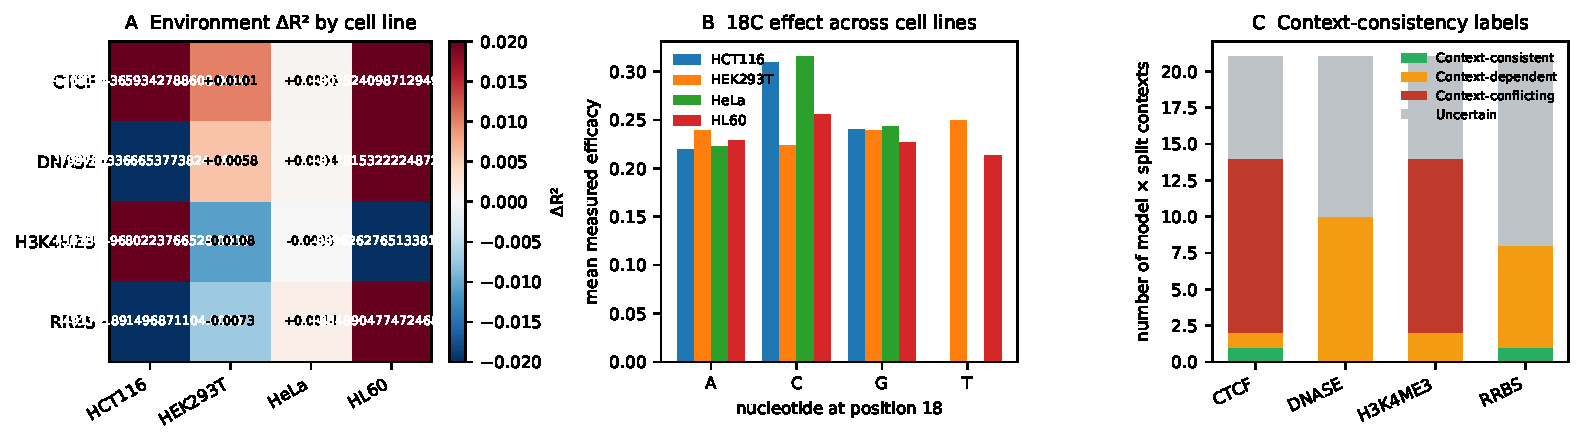
\includegraphics[width=\textwidth]{figures/fig6_cellline.pdf}
\caption{细胞背景下的效应异质性。\textbf{(A)} 各环境因子的平均 $\Delta R^{2}$ 按细胞系展开（排除发散行）。\textbf{(B)} 第 18 位碱基效应在四个细胞系中的方向与幅度（HCT116/HeLa 为正且较大，HL60 较小，HEK293T 反向）。\textbf{(C)} 按模型与划分统计的 cell-line context 标签分布：冲突与不确定占多数。}
\label{fig:cellline}
\end{figure}

\subsection{证据整合与生物学假设（E1--E4 汇总，无 E5/E6）}
\label{sec:res-evidence}

\textbf{问题与方法（RQ3）.} 如何把预测增量、模型归因、外部验证、反事实扰动与观测性关联组织为可比较、可追溯的证据，并据此排定后续实验的候选？

\textbf{观察 1（环境因素：四个因子全部为 Inconclusive）.} CTCF、DNase、H3K4me3、RRBS 均未通过 effect 门（$|\overline{\Delta R^{2}}|$ 为 $3.2\times10^{-4}$--$1.5\times10^{-3}$，门槛 0.01），跨模型 bootstrap 区间全部跨 0；CTCF 与 H3K4me3 另带 cell-line Context-conflicting 标签，DNase 与 RRBS 为 Uncertain。因此四者均判为 \textbf{Inconclusive}（表~\ref{tab:environment}、图~\ref{fig:evidence}）。

\textbf{观察 2（序列层面：四个非模型类一致，区域层级部分一致）.} 一致的部分是 PAM 邻近位置在位置层级被四个非模型类排在最高位（XGBoost/CNN/MLP/Transformer 的逐上下文峰值有 65.6\%--100\% 落在 17--20）；分歧的部分包括线性模型峰值在第 1 位（且把五模型平均谱的峰值拉到第 1 位）、Transformer 注意力与梯度/树归因不一致、以及 CNN/MLP 在区域汇总下更偏向种子核心区。这些分歧被保留为 model-dependent evidence，而不被平均掉。

\textbf{观察 3（本文证据链的收敛点：第 18 位的三方独立支持）.} 表~\ref{tab:convergence} 汇总第 18 位在六层证据框架中的位置。该位置是本文唯一同时获得 E2、E3、E4 三层独立支持的候选，且其中最关键的跨系统一致性（\S\ref{sec:res-external}）与无位置预设的饱和检验（\S\ref{sec:res-counterfactual}）均为本文新增。

\textbf{观察 4（其余候选）.} 除第 18 位外，按预设标准还筛出两类候选序列模式破坏（表~\ref{tab:candidates}）：C2 为 GAGG（出现在全部 3 个 CNN 核变体，carrier-vs-background 效应 $+0.012$，Fisher OR$=1.11$，BH-FDR$=0.031$），C3 为 GGGG（2 个核变体，效应 $+0.060$，OR$=1.38$，BH-FDR$=3.2\times10^{-5}$）。两者均仅在单一细胞系（HeLa）中达到富集显著（BH-FDR $<0.05$），故优先级低于 C1。

\textbf{统计证据.} 观察 1 的门槛与区间判定见 \S\ref{sec:methods-evidence}；观察 3--4 汇总的是已在各小节报告过的量，此处不引入新的检验。

\textbf{解释（假设）与边界：一个可证伪的生物学假设.} 综合上述，本文提出的假设是：

\begin{quote}
\emph{在本文数据所覆盖的 sgRNA 中，PAM 邻近区第 18 位的碱基身份与编辑效率存在关联，且该关联的方向在多个模型族与一个独立外部模型上一致；把第 18 位由 C 替换为 A 会降低编辑效率。该效应的大小依赖于细胞背景。}
\end{quote}

该假设的可证伪形式与最小扰动方案为：保持 sgRNA 其余 22\,nt 完全不变，仅替换第 18 位（C$\leftrightarrow$A），在同一实验体系中测定归一化编辑效率并做配对比较；预期方向为 C$>$A，预期效应量参考 E2 的观测差（HCT116/HeLa 约 $+0.09$）与 E4 的外部模型预测（$\Delta_{\text{CRISPRon}}=-12.43$ 分）。若配对实验显示方向相反或效应为零，则该假设被推翻。

必须强调其证据边界：\textbf{所有候选均为待验证假设，本文不包含任何湿实验验证。} 第 18 位的方向性结论由模型内部扰动（E4）与观测性碱基关联（E2）支持，\textbf{不构成因果证据}；模型归因的一致性（E3）也不等于生物学正确性——多个模型类一致只能说明它们依赖了相似的特征，不能排除它们共同依赖了数据中的混杂结构。这正是本文引入独立外部模型（E4）与饱和扰动的原因，也是这些证据仍止步于 E4 的原因。

\begin{table}[htbp]
\centering
\footnotesize
\caption{本文证据链的收敛点：第 18 位在六层证据框架中的支持情况。三方支持来自\textbf{互相独立}的证据来源（模型归因、外部模型扰动、实测标签关联），这是本文最强的计算证据组合；但缺少 E5（实验）证据，因此止步于假设。}
\label{tab:convergence}
\begin{tabular}{p{1.1cm}p{4.3cm}p{4.6cm}p{4.0cm}}
\toprule
层 & 该层对第 18 位的结论 & 关键数字 & 独立性来源 \\
\midrule
E1 & 不直接评价位置（评价整体预测能力） & 跨数据集 $R^{2}$：$0.067$--$0.120$ / $0.345$--$0.489$ / 全负 & 三个独立数据集 \\
\midrule
E2 & 第 18 位 C 组的实测效率高于 A 组（HCT116/HeLa/HL60） & $+0.090$ / $+0.092$ / $+0.027$；HEK293T $-0.015$（反转） & 实测标签，与模型无关 \\
\midrule
E3 & 四个非模型类（XGBoost/CNN/MLP/Transformer）的位置归因峰值集中在 PAM 邻近窗口 17--20 & 逐上下文峰值落在 17--20 的比例 65.6\%--100\%；单模型谱峰值分别为第 18、20、18、19 位。\textbf{Linear 例外}（21.9\%，峰值第 1 位） & 五类不同归纳偏置（\emph{但不独立于数据}） \\
\midrule
E4 & 本文 7 模型与独立外部模型 CRISPRon 对 C18A 的扰动方向 7/8 一致；饱和突变把第 18 位排 1/21 & $r=0.629$、$\rho=0.476$；C$\rightarrow$A 均值 $-12.425$ vs 其余 $+0.144$ & 独立第三方模型（不同数据、编码、尺度） \\
\midrule
E5 & \textbf{无} & --- & --- \\
\midrule
E6 & \textbf{不作断言} & --- & --- \\
\bottomrule
\end{tabular}
\end{table}

\begin{figure}[htbp]
\centering
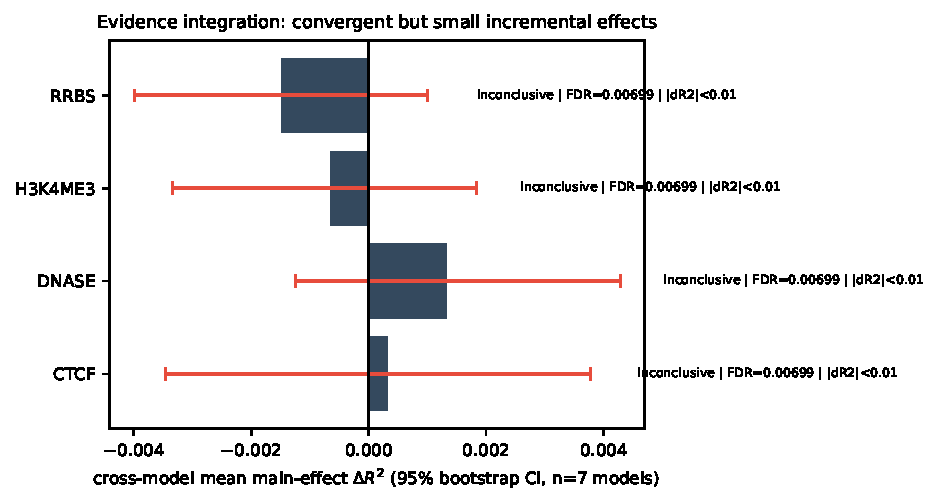
\includegraphics[width=0.8\textwidth]{figures/fig7_evidence.pdf}
\caption{证据整合：环境因子的跨模型平均主效应与 95\% bootstrap 区间，并标注证据等级。四个因子全部为 Inconclusive，且 $|\Delta R^{2}|$ 均小于 0.01。Importance--$\Delta R^{2}$ 辅助视图见补充图~\ref{fig:importance}。}
\label{fig:evidence}
\end{figure}

\begin{table}[htbp]
\centering
\footnotesize
\caption{Candidate hypotheses prioritised from the existing results for minimal follow-up perturbation experiments. No wet-lab validation was performed in this study; effects are model-derived or measured associations, not causal estimates.}
\label{tab:candidates}
\begin{tabular}{lrrrrrr}
\toprule
candidate & type & multi\_model\_support & effect & robustness & minimal\_perturbation & priority \\
\midrule
C1: position-18 base substitution & single-nucleotide & 3/5 models place position 18 in top-3 in >=65% of runs; PAM-proximal seed region is the highest region for 2/5 & mean efficacy C-A: HCT116 +0.090, HeLa +0.092, HL60 +0.027, HEK293T -0.015 & cell-line CNNs: |dR| for C->A is larger in HCT116 (0.016-0.084) and HeLa (0.028-0.090) than HEK293T (0.003-0.007) and HL60 (0.002-0.017) & substitute position 18 (C<->A) keeping the rest of the sgRNA fixed & high \\
C2: GAGG candidate pattern (enriched) & motif disruption & shared by CNN k=3/5/7 contexts (12 contexts) & carrier-vs-background effect +0.012; OR=1.11 & BH-FDR=0.031 (motif\_enrichment family); single cell line (HeLa) & disrupt the 4-nt core inside the PAM-proximal window & medium \\
C3: GGGG candidate pattern (most enriched) & motif disruption & CNN contexts (2 contexts: k=3, k=7) & carrier-vs-background effect +0.060; OR=1.38 & BH-FDR=0.0000; single cell line (HeLa) & disrupt the GGGG core & medium \\
reference: CTGG (highest support, not enriched) & motif disruption & highest seqlet support (1273) & carrier-vs-background effect -0.046; OR=0.83 & BH-FDR=1 (not significant in this batch) & not prioritised: support without enrichment & low \\
\bottomrule
\end{tabular}
\end{table}

% 本文件由 analysis/reporting/paper_rewrite/build_rewrite_tables.py 自动生成。
% 请勿手工编辑；数字来源见文件头注释与 results/paper_rewrite/authoritative_numbers.json。
\begin{table}[htbp]
\centering
\footnotesize
\caption{本文使用的\textbf{六层证据}分类。每一层回答不同的问题、有不同的失效模式，且\emph{不能相互替代}：低层证据不能升级为高层证据，高层证据的存在也不能反推低层证据。全文每一处结论均在括号中标注其所属层（E1--E6）。本文\textbf{不含任何 E5 证据}，因此不产生任何 E6 层面的因果断言。}
\label{tab:evidence-layers}
\begin{tabular}{p{0.5cm}p{2.6cm}p{3.4cm}p{4.2cm}p{3.6cm}}
\toprule
层 & 名称 & 回答的问题 & 本文中的实例 & 该层\textbf{不能}支持 \\
\midrule
E1 & 预测证据 & 模型能否在未见样本上预测标签？ & 测试集 $R^{2}$/Pearson/Spearman；跨数据集复现；CRISPRon 的 WT/C18A 评分差 & 因果；机制；模型"理解"了生物学 \\
\midrule
E2 & 关联证据 & 标签与某可观测属性是否同变？ & 第 18 位 C 与 A 分组的实测效率差（按细胞系）；GC 含量与效率的相关系数 & 因果；方向性机制；对该属性的干预效应 \\
\midrule
E3 & 归因证据 & 模型输出依赖输入的哪些部分？ & 线性系数、TreeSHAP、IG、CNN 逐位点归因、注意力 & 统计显著性；生物学重要性；因果 \\
\midrule
E4 & 反事实证据 & \emph{模型}在输入被扰动后如何响应？ & 符号化 ISM（第 18 位 C$\rightarrow$A/G/T）；逐位点饱和突变；候选模式破坏 & 真实编辑效率的变化；实验可验证的效应量 \\
\midrule
E5 & 实验证据 & 真实实验中扰动是否改变结果？ & \textbf{本文无}（见 \S\ref{sec:future} 的预登记实验设计） & 超越所测体系的外推 \\
\midrule
E6 & 因果证据 & 干预是否在该体系中导致效应？ & \textbf{本文不作任何此类断言} & --- \\
\bottomrule
\end{tabular}
\end{table}

